\documentclass[12pt]{article}
\usepackage{listings}
\usepackage{graphicx}
\usepackage{xcolor}

\begin{document}
\title{ECEC 471 Lab 4}
\author{Nicholas Sica}
\date{November 6, 2020}
\maketitle

\section{Introduction}
\subsection{Overview}
\subsection{Invert Chain}
An inverter chain is, like the name implies, a chain of inverters used to reduce propagation delay by setting
the number of stages to be able to efficiently run the circuit, given a certain input and ouput capacitance.
If there are too many stages, the inverter chain could end up doing more harm than help. Using Equation~\ref{eq:p_inv}
and using the value of 0.5 for $p_{inv}$ we can solve for $\rho$. Then using Equation~\ref{eq:num_stages} we can solve
for the best number of stages for the inverter chain. The number that was achieved by this method for $\rho$ was about
3.181. The best number of stages was about 3.381 which was rounded to three. 
\begin{equation} \label{eq:p_inv}
    p_{inv} + \rho(1 - \ln\rho) = 0
\end{equation}
\begin{equation} \label{eq:num_stages}
    N = \log_{\rho}{\frac{C_{out}}{C_{in}}}
\end{equation}
Working backwards using Figure~\ref{eq:c_in}
The output and input capacitances for each stage can be found which leads us to multiply th previous stage transistor
widths by 3.69 to get the transistor sizes for the current stage.
\begin{equation} \label{eq:c_in}
    C_{in} = \frac{C_{out} \times g}{\hat{f}}
\end{equation}
\subsection{Ring Oscillator}
A ring oscillator is a chain of inverters with the input and output tied together. A ring oscillator is used in digital
logic to deliver a clock signal to the circuit. The period of a signal is the time it takes for one cycle to pass. It usually
is ideal to get the time it takes for a bunch of cycles to pass and divide by the number of cycles you took.
\section{Simulation and Analysis}
\subsection{Schematic Design}
Figure~\ref{fig:inv_chain_schem} shows the transistor-level schematic of the inverter chain. It was a straight-forward
schematic with just the number of inverters needed for minimum delay, three in this case. Figure~\ref{fig:inv_chain_sim}
shows the simulation schematic with the source and load of 0.1fF and 5fF as specified in the lab.
A pulse is used so we can measure the propagation delay of each inverter in the chain as well as the propagation delay
of the whole chain. The pulse has an amplitude of 1.2V, a period of 20ns, a rise time of 10ps, a fall time of 10ps and
a pulse width of 10ns.
\begin{figure}[!htb]
    \centering
    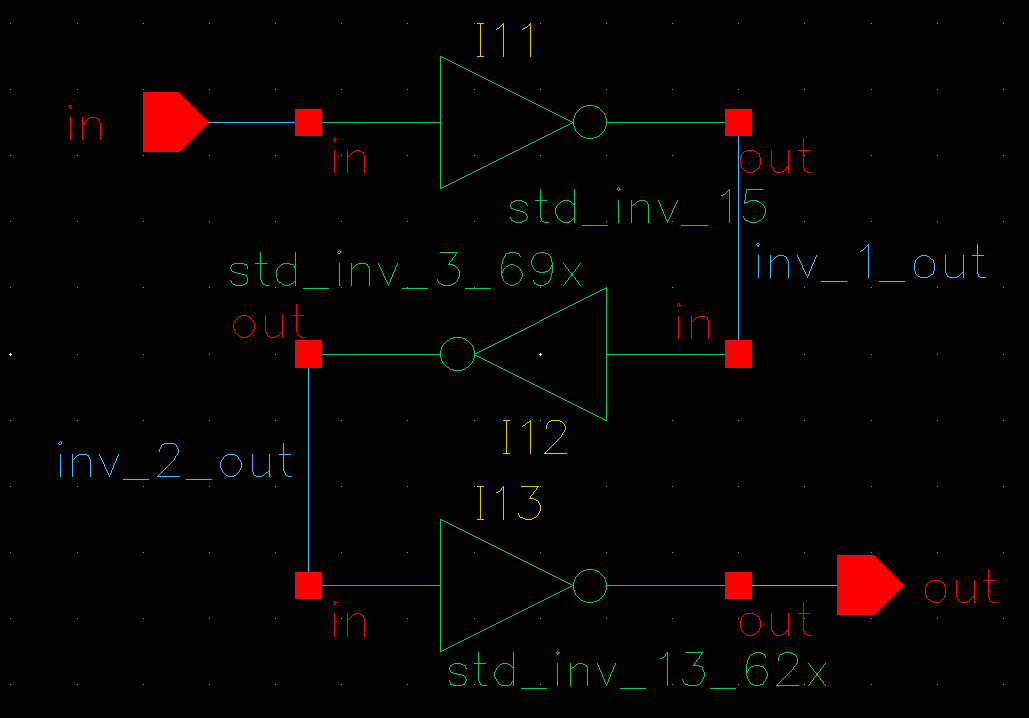
\includegraphics[width=4in]{figures/inv_chain_schem.png}
    \caption{Transistor-level Inverter Chain Schematic}\label{fig:inv_chain_schem}
\end{figure}
\begin{figure}[!htb]
    \centering
    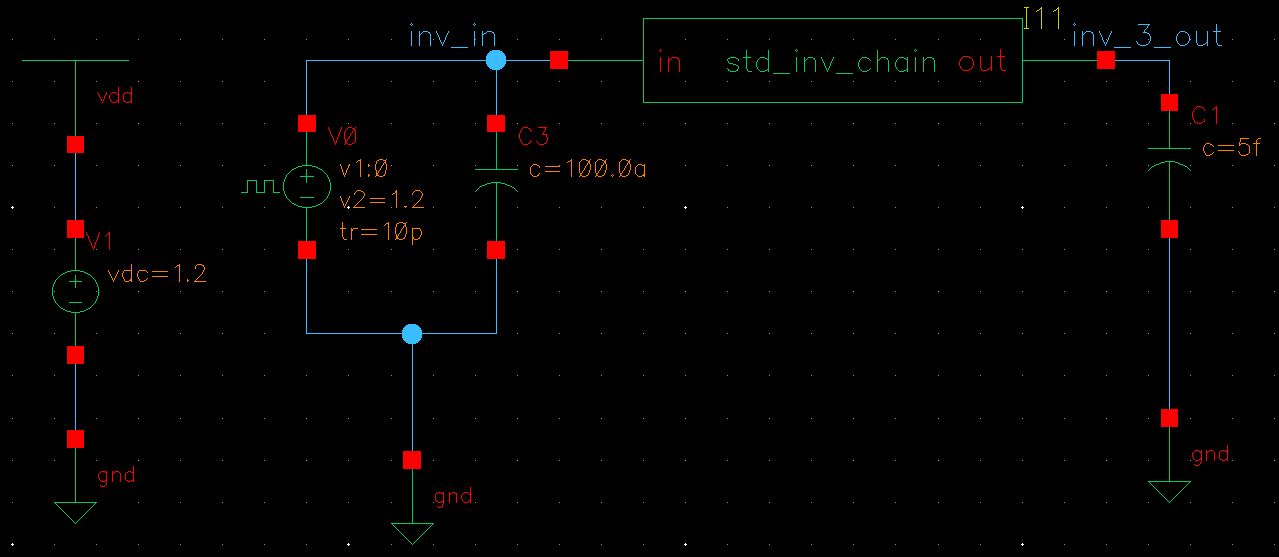
\includegraphics[width=5in]{figures/inv_chain_sim.png}
    \caption{Inverter Chain Simulation Schematic}\label{fig:inv_chain_sim}
\end{figure}

The transient analysis of the circuit is shown in Figure~\ref{fig:inv_chain_tran}. Using the transient analysis graphs,
the propagation delay of the entire chain was found to be 25.05ps, while each the first, second, and third
inverters' propagation delays are 8.95ps, 10.47ps, and 5.63ps, respectively. In lab two, the propagation delay was found to be
25.68ps which is a bit larger than the propagation delay of our inverter chain.
\begin{figure}[!htb]
    \centering
    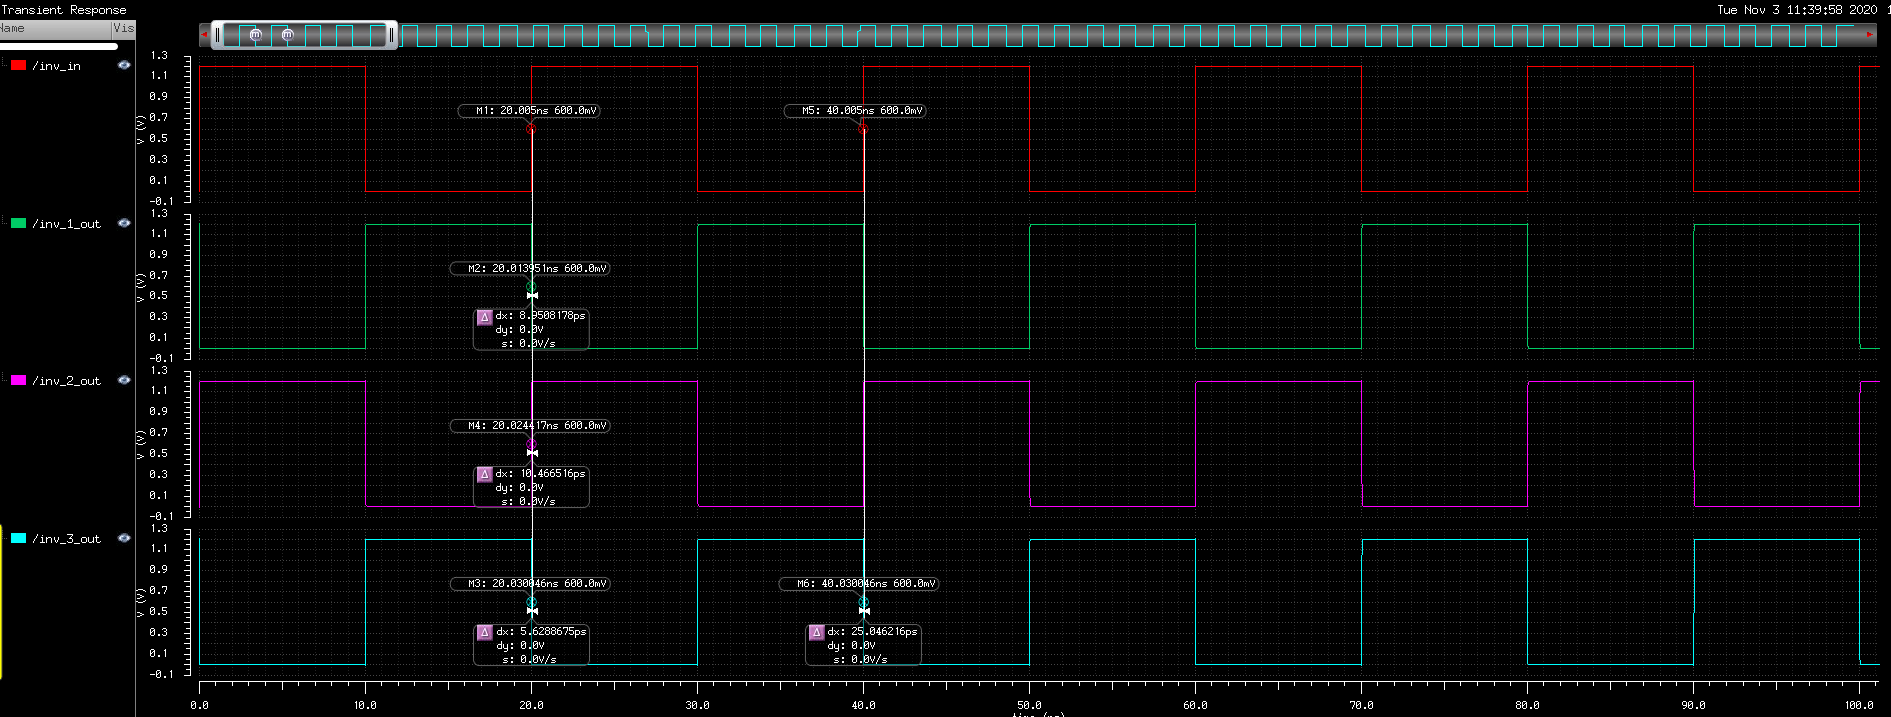
\includegraphics[width=5in]{figures/inv_chain_tran.png}
    \caption{Inverter Chain Transient Analysis}\label{fig:inv_chain_tran}
\end{figure}

After layout was done, parasitic extraction was done and simulation was re-run with the parasitics factored in. 
Figure~\ref{fig:inv_chain_post_layout_tran} was used to find the propagation delay at all stages is about 2ps longer
while the entire chain is about 6ps longer. 
\begin{figure}[!htb]
    \centering
    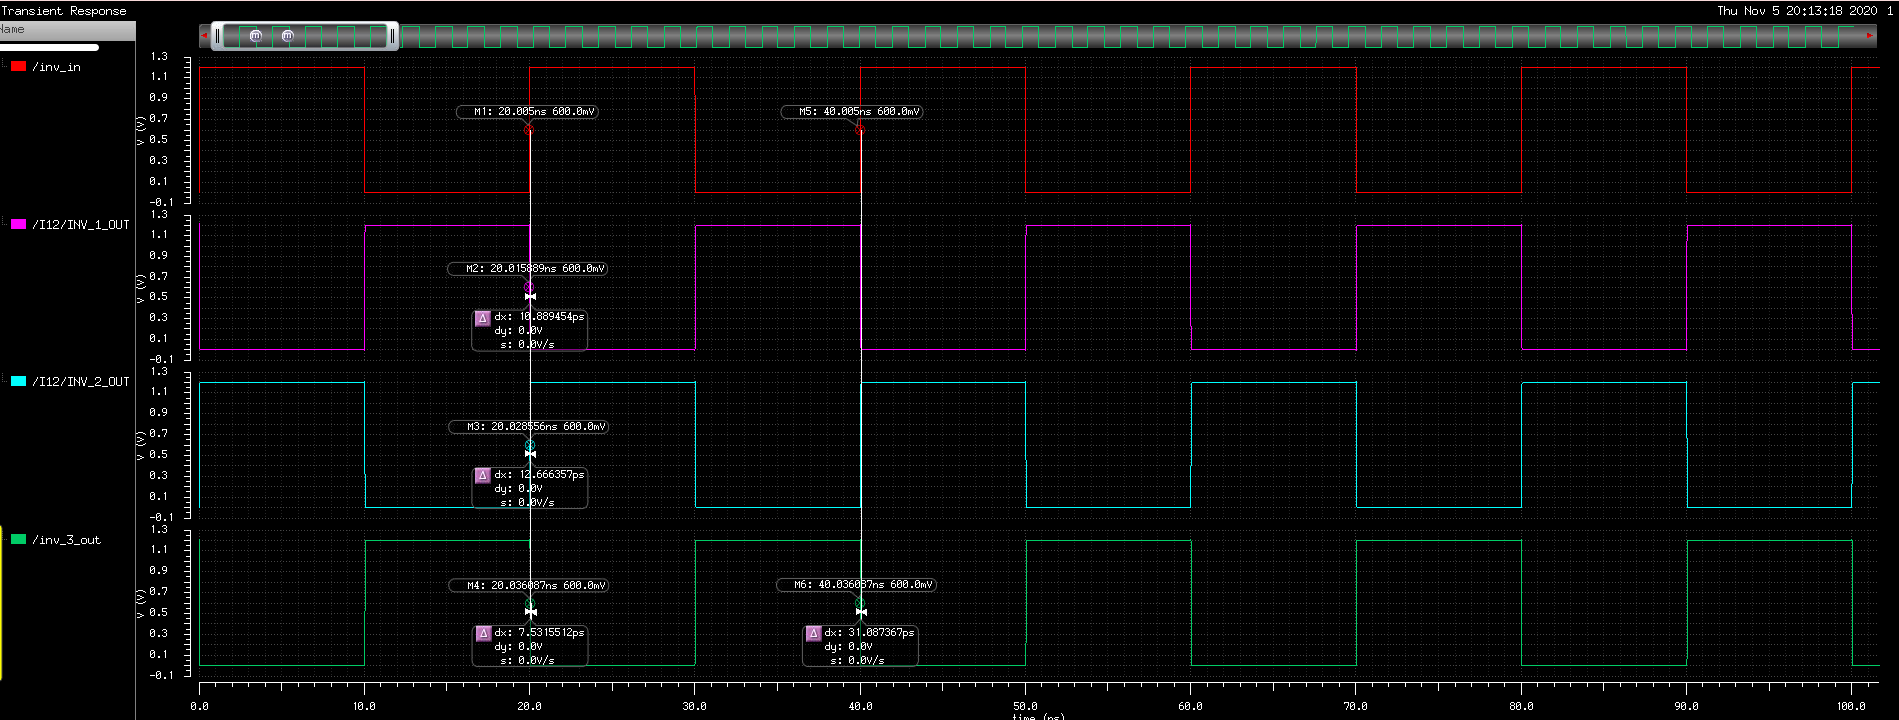
\includegraphics[width=5in]{figures/inv_chain_post_layout_tran.png}
    \caption{Inverter Chain Post-Layout Transient Analysis}\label{fig:inv_chain_post_layout_tran}
\end{figure}

The ring oscillator schematic is shown in Figure~\ref{fig:ring_osc_schem} and is simply twenty-one inverters with the
output tied to the input of the entire chain. Afterwards, simulation was setup as shown in Figure~\ref{fig:ring_osc_sim}
and is similar to the layout of all the other simulations.
\begin{figure}[!htb]
    \centering
    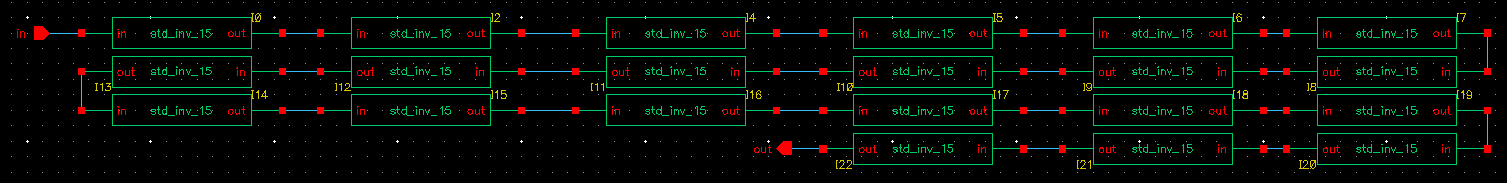
\includegraphics[width=5in]{figures/ring_osc_schem.png}
    \caption{Transistor-level Ring Oscillator Schematic}\label{fig:ring_osc_schem}
\end{figure}
\begin{figure}[!htb]
    \centering
    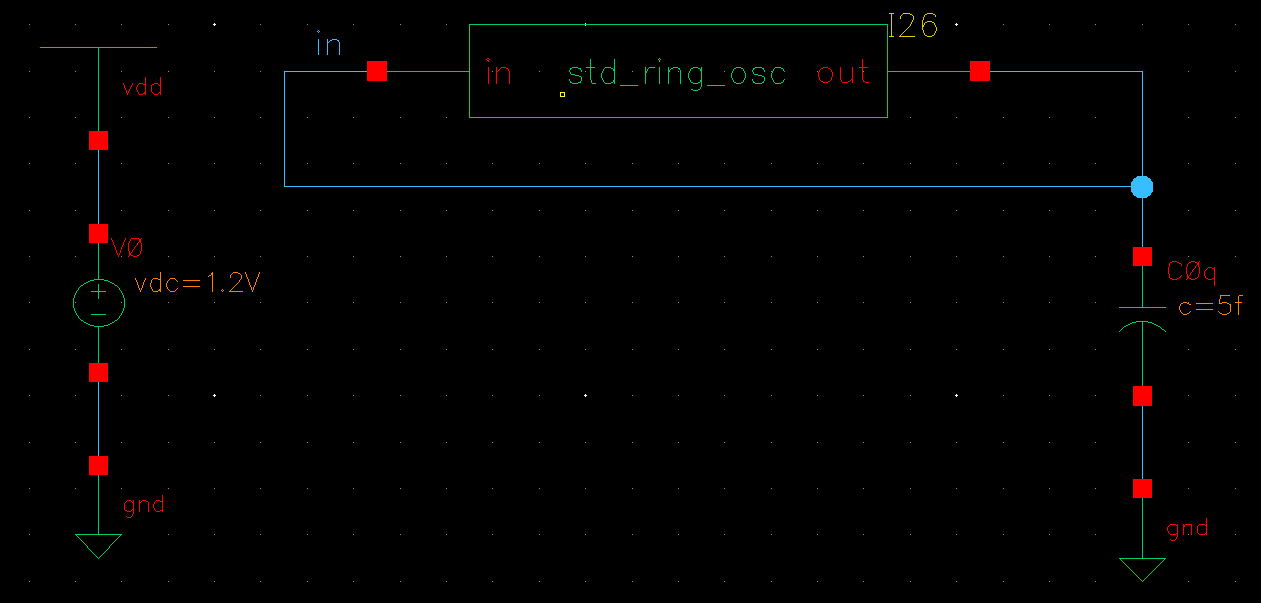
\includegraphics[width=5in]{figures/ring_osc_sim.png}
    \caption{Ring Oscillator Simulation}\label{fig:ring_osc_sim}
\end{figure}

Lastly, simulation was run and Figure~\ref{fig:ring_osc_tran} was obtained. With this we were able to count twenty-nine
cycles and get a delay of 7.81ns over those twenty-nine cycles. Using that information, a frequency of 3.71GHz or a period of
0.27ns was obtained.
\begin{figure}[!htb]
    \centering
    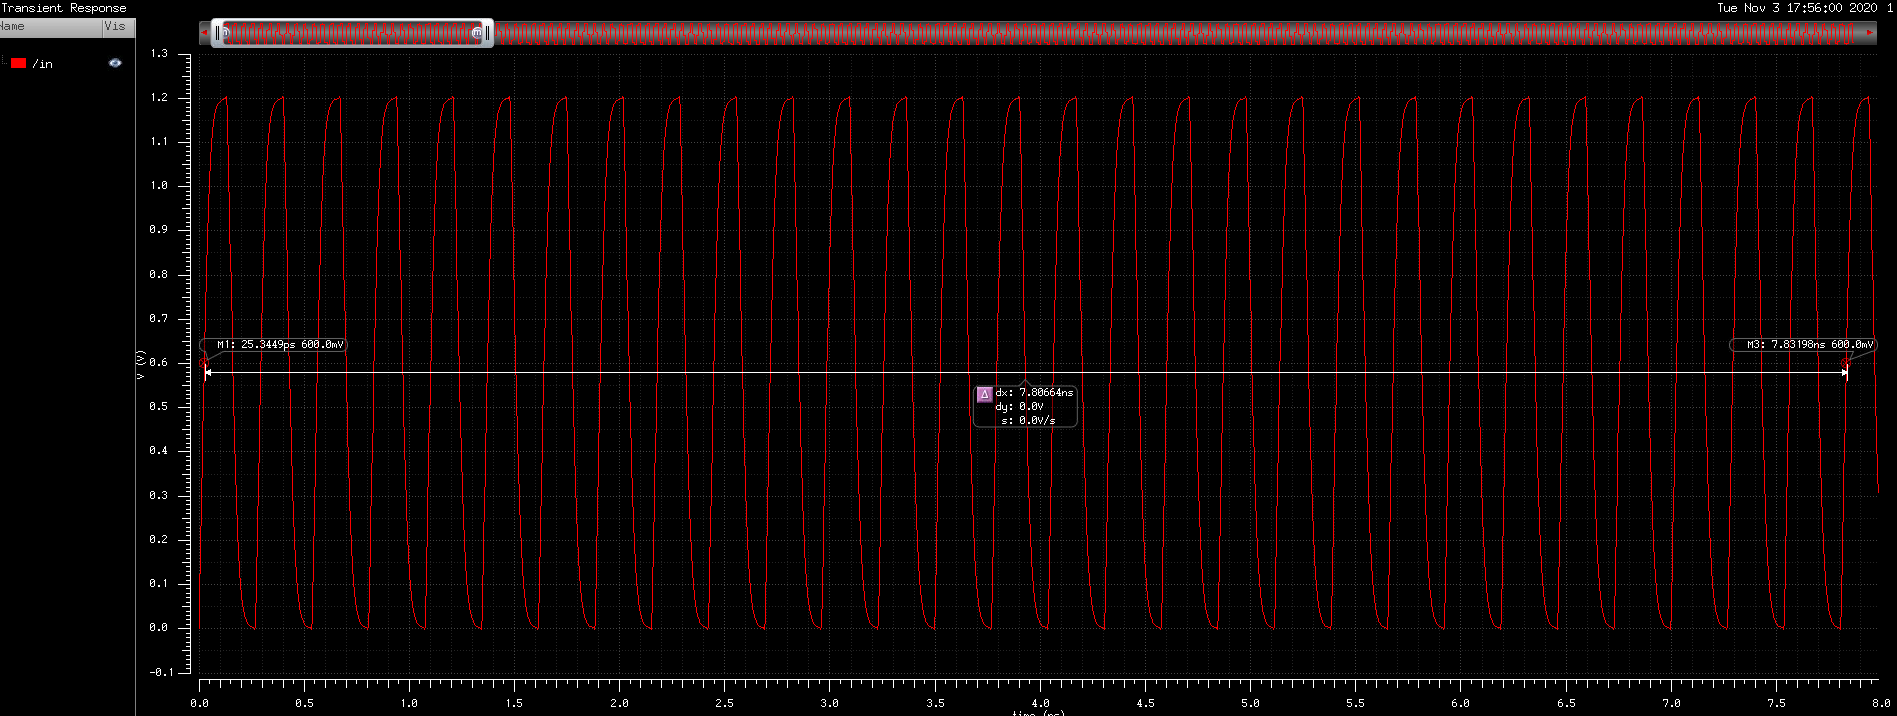
\includegraphics[width=5in]{figures/ring_osc_tran.png}
    \caption{Ring Oscillator Transient Analysis}\label{fig:ring_osc_tran}
\end{figure}
\subsection{Inverter Chain Layout Design}
After the inverter chain's schematic was finished, layout was done as shown in Figure~\ref{fig:layout}. This time, the pitch of
each sized inverter was matched to
ensure smooth integration into the inverter chain. In order to achieve this, "fingers" were used to allow for a smaller implant
width, but still keep the desired width intact.
\begin{figure}[!htb]
    \centering
    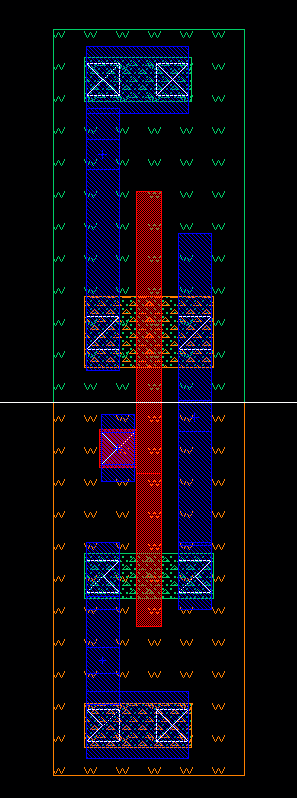
\includegraphics[width=5in]{figures/layout.png}
    \caption{Inverter Chain Layout}\label{fig:layout}
\end{figure}

Lastly, design rule checking(DRC) is used to make sure that no design rules are being violated and everything is fixed very painstakingly.
The results for the DRC can be seen in Figure~\ref{fig:drc}  After that layout versus schematic(LVS) was used to make sure our layout matches
the design we modeled with the schematic and can be seen in Figure~\ref{fig:lvs}. Once LVS was done, we used parasitic extraction to get
the parasitics of the circuit and do post-layout simulation.
\begin{figure}[!htb]
    \centering
    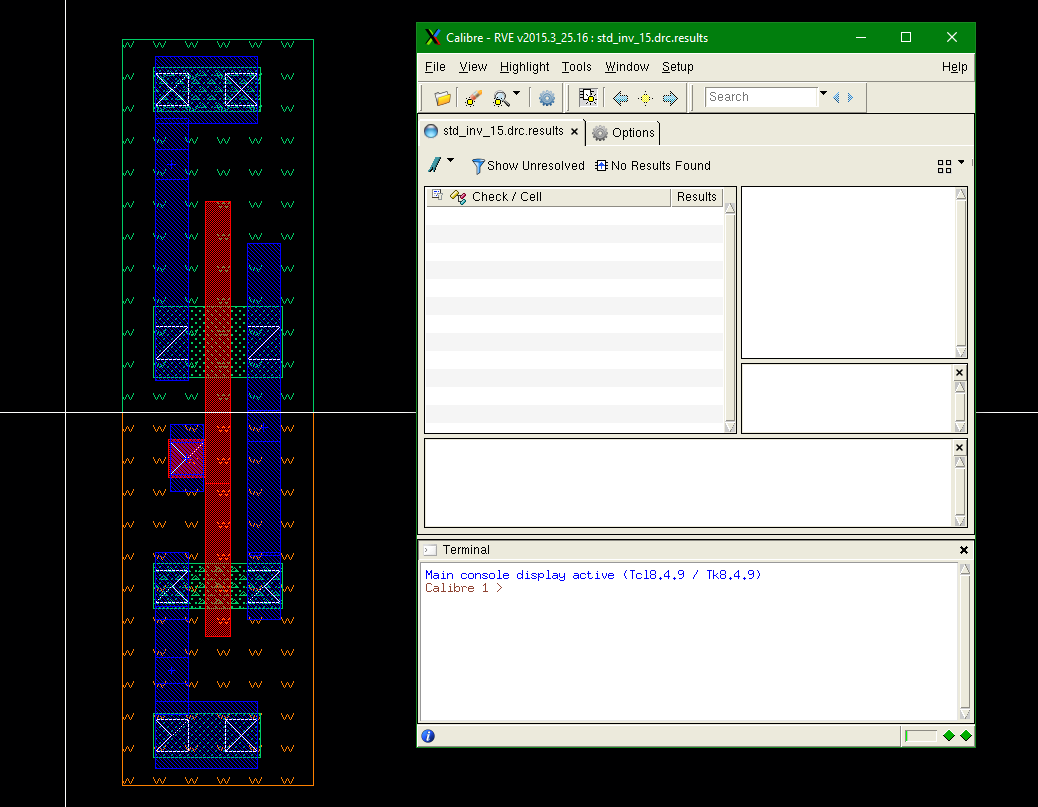
\includegraphics[width=3.5in]{figures/drc.png}
    \caption{DRC Results}\label{fig:drc}
\end{figure}
\begin{figure}[!htb]
    \centering
    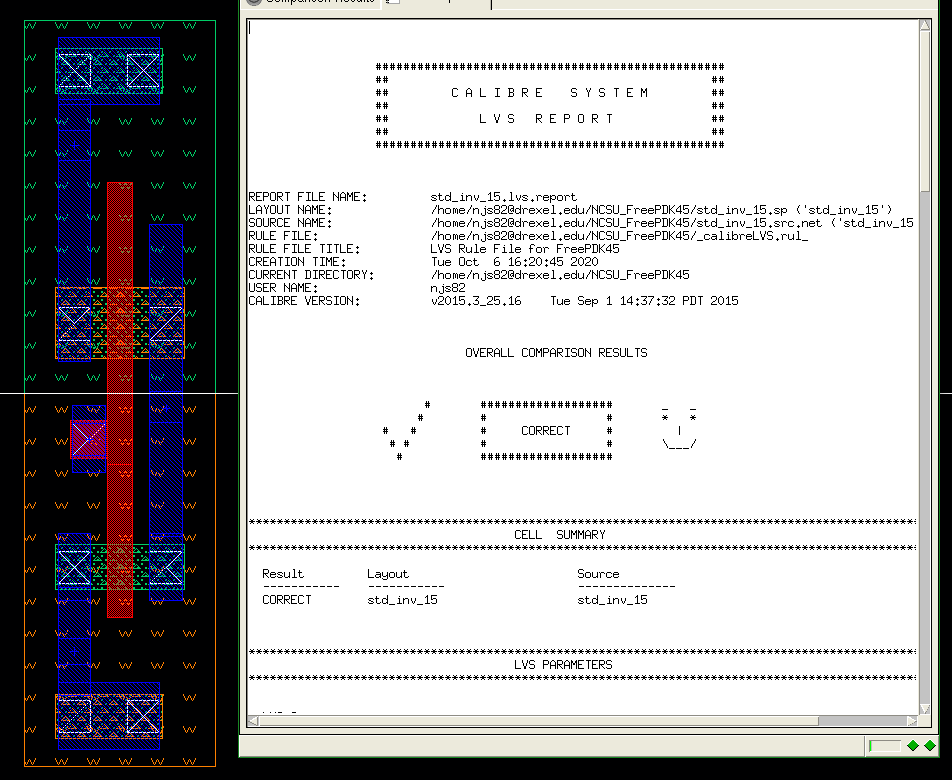
\includegraphics[width=3.5in]{figures/lvs.png}
    \caption{LVS Results}\label{fig:lvs}
\end{figure}
\clearpage
\section{Conclusion}
The lab helped the class figure out how to currectly size gates to achieve minimum delay and work through the issues of pitch matching
to get all the pieces of a circuit to fit together nicely. The parasitic extraction tool was a pain to wrestle with, mostly due to a
bug on Cadence's end. Everything came out as expected with the inverter chain speeding up the circuit a bit.
\end{document}
%%% Local Variables:
%%% mode: latex
%%% TeX-master: t
%%% End:
